\section{Methodology}
\subsection{Data Preprocessing:}
\begin{itemize}
	\item Silence and Noise Removal\\
	Doing a spot check on both training and testing set, we discovered that there exists silence or noise at the beginning of most audio files. We removed those silence or noise parts by calculating the average loudness of each audio file, and recursively comparing the value of 30\% of average loudness to first $\frac{3}{4}$ of the audio file.\\
	\item Equalizing Loudness:\\
	We also figured out that ,between training set and testing sets, there is a loudness difference not representative of class label. So, we linearly equalized average loudness of each file by the average loudness of all audio files. \\
\end{itemize}
\subsection{Feature Extraction:}
	We utilized general audio features: Zero Crossing Rae, Energy, Entropy of Energy, Spectral Centroid, Spectral Entropy, Spectral Spread, Spectral Entropy, Spectral Flux, Spectral Rolloff,  MFCCs, Chroma Vector and Chroma Deviation. The library we used for those feature extractions are pyAudioAnalysis\cite{b1}.\\
	After analyzing the dataset, we also noticed that number of local minimum amplitude peaks is one representative feature and we added that to feature list.\\
\subsection{Model Selection:}
	Our whole model-building infrastructure is based on scikit-learn\cite{b2}\cite{b3}. \\
	We tried K-Nearest Neighbor, Support Vector Machine, Boosting, Random Forest, Extratrees, Multiple Instance Learning, Label Propagation. After few experiments, it seemed like tree algorithms performed poorly on this task and we finalized our focus on SVM, Label Propagation, SVC and MILR with pipeline. This classifier undercalled Normal and Neoplasm patients, which we think is resulted from different class distributions between training and testing set. So, we converted this relatively complex learning task into three less complicated tasks: Normal vs. Pathological, Vocal vs. Rest of Diseases, and Phonotrauma vs. Neoplasm.[Fig. 1.] The reason why we design the pipeline this way is based on the difficulty of classification. (From easiest Normal vs. Pathological to hardest Phonotrauma vs. Neoplasm)
	\begin{figure}[htbp]
		\begin{center}
			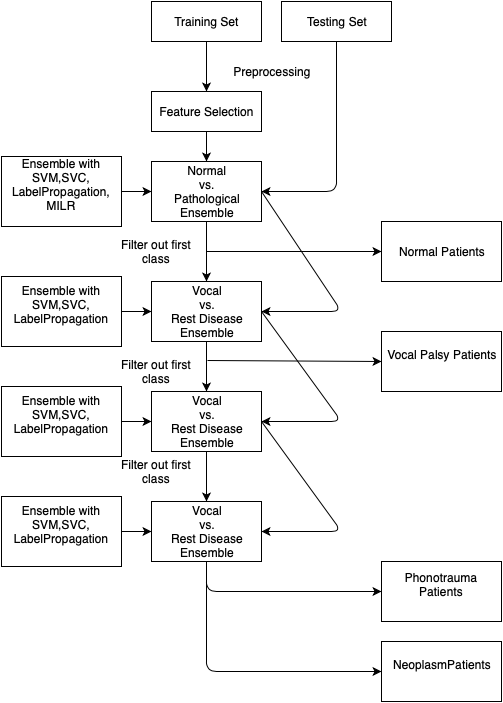
\includegraphics[scale=0.35]{Diagram_1.png}
		\end{center}
		\caption{Pipeline Ensemble}
	\end{figure}
	\subsection{Hyper Parameter Tuning:}
		Since the size of training set is getting smaller and smaller as we propagate through the pipeline, in order to get trustworthy accuracy to tune parameter for SVC, for all three ensembles, we use the same parameter tuned in the first ensemble. The process is pretty straightforward; we simply set up two loops, one of which for C and one of which for gamma. The tuned parameters are 10 for C, and 0.01 for gamma. Also due to the skewed distribution in training set, we modify the class weight with respect to the proportion of class. 

